%--------------------------------------%
%----- 3_Versuchsdurchführung.tex -----%
%--------------------------------------%
%--------------------------------------%
%
\subsection{Messung}
\label{subsec:3_Messung}
%

%
\begin{figure}[H]
  \Large
  \centering
  \begin{tikzpicture}[circuit ee IEC, font = \sffamily]
    \matrix(M)[
      matrix of nodes, nodes in empty cells,
      inner sep = 0pt, outer sep = -.1\pgflinewidth,
      column sep = 20mm, row sep = 15mm,
      nodes = {minimum width = 0pt}
      ]
    {
      & & & & & \\
      & & & & & \\
      & & & & & \\
      & & & & & \\
      & & & & & \\
    };
    %
    \draw[circuit symbol unit = 15pt]
      (M-2-2) to [voltage source] (M-5-2);
    \draw[circuit symbol unit = 15pt]
      (M-2-2) to [resistor = {info = $R$, info' = \SI{1}{\kilo\ohm}}] (M-2-6);
    \draw[circuit symbol unit = 15pt]
      (M-2-6) to [capacitor = {info = $C$, info' = \SI{100}{\nano\farad}}] (M-5-6);
    %
    \draw (M-5-2)--(M-5-6);
    %
    \draw[UPfeil = 6mm]
      ([xshift = -9mm]M-2-2.east)--([xshift = -9mm]M-5-2.east)
      node[midway, left]{$U_\mathrm{E}$};
    \draw[UPfeil = 16mm]
      ([yshift = 13mm]M-2-2.south)--([yshift = 13mm]M-2-6.south)
      node[midway, above]{$u_\mathrm{R}$};
    \draw[UPfeil = 6mm]
      ([xshift = 14mm]M-2-6.west)--([xshift = 14mm]M-5-6.west)
      node[midway, right]{$u_\mathrm{C}$};
    \draw[IPfeil = 4mm]
      ([xshift = 6mm]M-2-2.center)--([xshift = 6mm]M-2-3.center)
      node[midway, above]{$i$};
    %
  \end{tikzpicture}
  \caption{Schaltbild der untersuchten RC-Reihenschaltung}
  \label{fig:3_Schaltung}
\end{figure}
%
%
%
\newpage
\subsection{Simulation}
\label{subsec:3_Simulation}
%
Im Anschluss an den praktischen Versuchsteil wurde die RC-Reihenschaltung in der frei verfügbaren Simulationssoftware LTspice\footnote{siehe \cite{src:LTspice}} nachgebaut und um ein weiteres RC-Glied erweitert. Dabei wurden die gleichen Bauteilwerte von $R = \SI{1}{\kilo\ohm}$ und $C = \SI{100}{\nano\farad}$ verwendet. Am Eingang der Schaltung wurde~--~analog zur Messung~--~eine Rechteckspannung $u_\mathrm{E}$ angelegt. Die Einstellwerte für die Spannungsquelle sind in Abb. \ref{fig:3_Sim_Spannungsquelle} dokumentiert.
%
\begin{figure}[H]
  \centering
  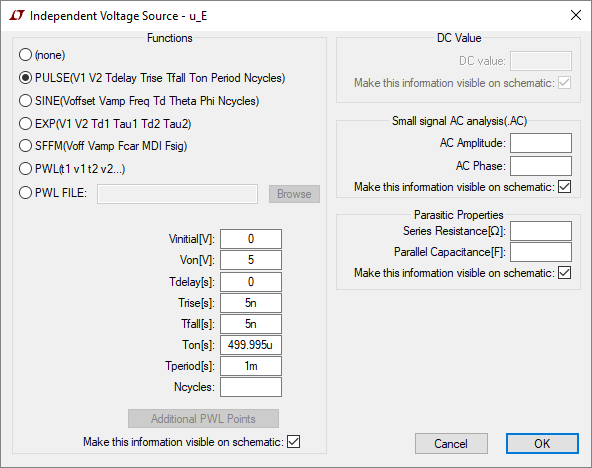
\includegraphics[width=0.9\linewidth]{src/3_Sim_Spannungsquelle.png}
  \caption{Simulation: Einstellwerte der Spannungsquelle}
  \label{fig:3_Sim_Spannungsquelle}
\end{figure}
%
Die resultierende Simulationsschaltung ist in Abb. \ref{fig:3_Sim_Schaltung} dargestellt. Darin befindet sich neben den passiven Bauelementen und der Spannungsquelle auch ein Masse-Element zur Festlegung des Bezugspotentials. Messgeräte zur Erfassung der gewünschten Zustandsgrößen müssen in LTspice nicht gesondert eingefügt werden; die Simulation umfasst immer alle vorhandenen Zustandsgrößen.
%
\begin{figure}[H]
  \centering
  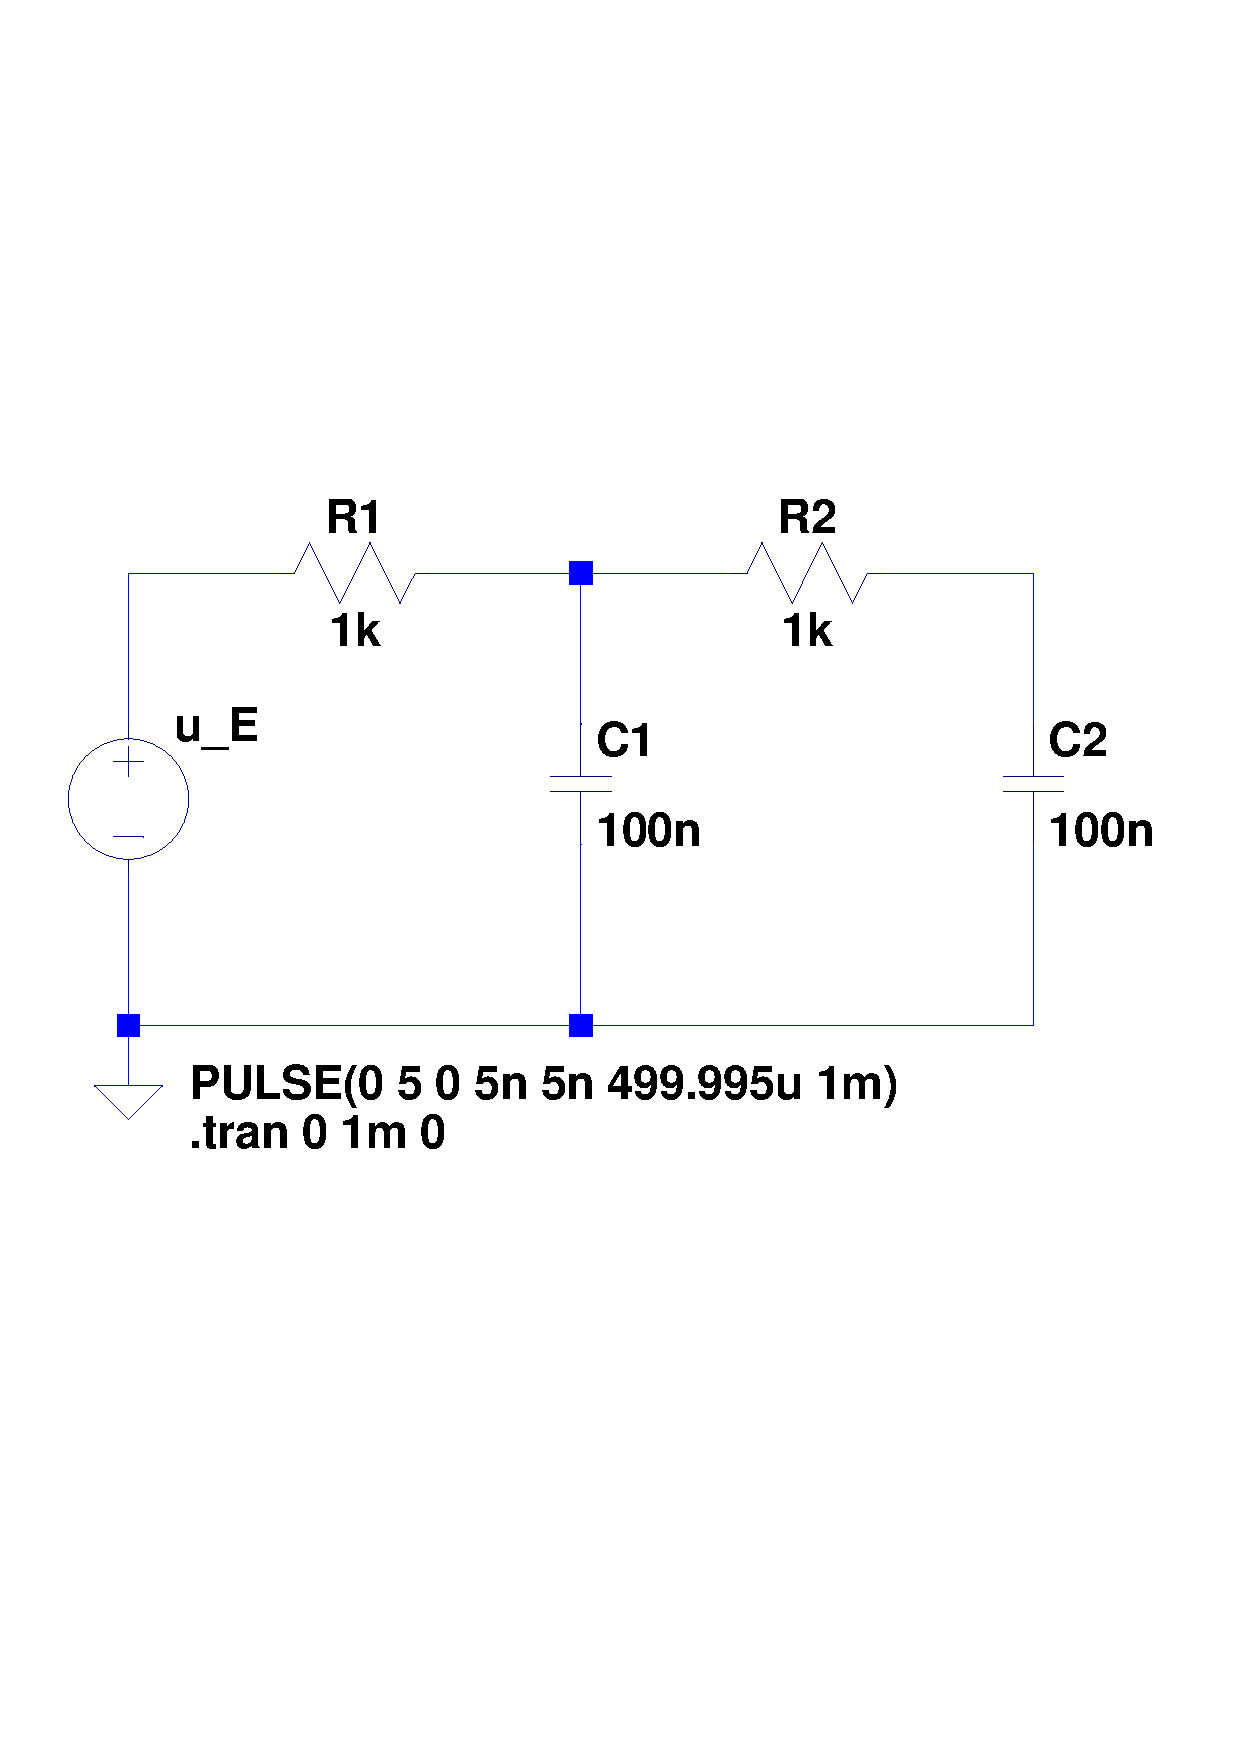
\includegraphics[width=0.6\linewidth]{src/3_Sim_Schaltung.pdf}
  \caption{Simulation: Schaltung in LTspice}
  \label{fig:3_Sim_Schaltung}
\end{figure}
%
Im Rahmen der Simulation wurde die Schaltung für eine Periode simuliert. Dabei erfolgte zunächst das Zuschalten der Quelle, danach das Abschalten. Die Flankenzeiten wurden mit $T_\mathrm{rise} = T_\mathrm{Fall} = \SI{1}{\milli\second}$ vorgegeben. Die entsprechenden Einstellungen sind Abb. \ref{fig:3_Sim_Parameter} zu entnehmen.
%
\begin{figure}[H]
  \centering
  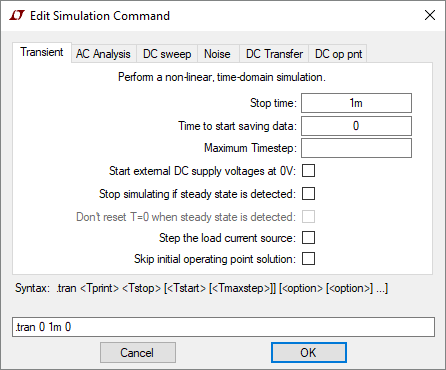
\includegraphics[width=0.7\linewidth]{src/3_Sim_Parameter.png}
  \caption{Simulation: Einstellwerte der Simulationsparameter}
  \label{fig:3_Sim_Parameter}
\end{figure}
%
Im Anschluss an die Simulation wurden die Ergebnisse aus LTspice exportiert und mit Hilfe der readLTspice-Funktion\footnote{siehe \cite{src:readLTspice}} in Matlab eingelesen. Dort wurden die Daten ausgewertet.
%
%
%